\RequirePackage{plautopatch}

\documentclass[a4paper, 11pt]{ltjsarticle}


% マージン設定
\usepackage[top=20mm, bottom=20mm, left=25mm, right=15mm]{geometry}

% LuaLaTeX用日本語対応パッケージ
\usepackage{luatexja}
\usepackage{luatexja-fontspec}

% 必要なパッケージ
\usepackage{fontspec}
\usepackage{titlesec}
\usepackage{graphicx}
\usepackage{amsmath}
\usepackage{amssymb}
\usepackage{mathtools}
\usepackage{tocloft}
\usepackage{indentfirst}
\usepackage{tikz} % カスタム点線用
\usepackage{here}
\usepackage{subcaption}
\usepackage{bookmark}
\usepackage{booktabs}
\usepackage{multicol}
\usepackage{multirow}
\usepackage{flushend}
\usepackage{threeparttable}
\usepackage{enumitem}
\usepackage{pifont}  % 丸囲み数字を使うためのパッケージ
\usepackage{url}
\usepackage{svg}
\usepackage{makecell}
\hypersetup{hidelinks}
\usepackage[numbers]{natbib}

% 図:1のコロンを消す
\captionsetup{labelsep=space}

% 参考文献を上付きにする
\usepackage[super]{cite}
\renewcommand\citeform[1]{[#1]}

\setlength{\baselineskip}{14pt}
\setlength{\parindent}{1\zw}

\titleformat{\section}{\large\bfseries}{\thesection.}{1\zw}{}
\titleformat{\subsection}{\large\bfseries}{\thesubsection.}{1\zw}{}
\titleformat{\subsubsection}{\large\bfseries}{\thesubsubsection.}{1\zw}{}

\setcounter{tocdepth}{3}
\makeatletter
\renewcommand{\numberline}[1]{#1.~}
\renewcommand{\cftsecleader}{\cftdotfill{\cftdotsep}}
\renewcommand{\cftsubsecleader}{\cftdotfill{\cftdotsep}}
\renewcommand{\cftsubsubsecleader}{\cftdotfill{\cftdotsep}}
\makeatother

\DeclareCaptionFont{designatedFont}{\fontsize{11pt}{14pt}\selectfont}
\captionsetup{font=designatedFont}

%---ここから中身---------------------------------------------------------------------------------------
\begin{document}
\fontsize{11pt}{14pt}\selectfont

%---表紙---------------------------------------------------------------------------------------
\thispagestyle{empty}
\begin{center}
\pagenumbering{gobble}  %ページ番号をカウントしない

\vspace*{40mm}
{\huge\noindent 災害時を想定したアドホックネットワーク}\\
\medskip
{\huge\noindent 構築手法の検討}\\
\vspace{\baselineskip}
{\huge\noindent\textbf{Study of Construction Methods for Ad-Hoc Network under Disaster}}\\
\vspace{120mm}

{\huge\noindent
2025年3月4日\\
東京都立産業技術高等専門学校\\
ものづくり工学科 情報通信工学コース \\
末廣 隼人\\
指導教員 髙﨑 和之    \\
}
\vspace{40mm}

\end{center}

%---目次------------------------------------------------------------------------------------------
\clearpage  %新しいページの追加
\thispagestyle{empty}
\tableofcontents  %目次の自動生成 目次をクリックするとその章,節に飛ぶことができる

%---はじめに---------------------------------------------------------------------------------------
\clearpage
\pagenumbering{arabic}
\section{はじめに}
日本では地震をはじめ,台風や豪雨などの自然災害が発生しており,その影響でネットワークが使用不能に
なる可能性がある.特に,大規模災害時に通信インフラへのアクセス集中や通信基地局の損壊等により,
ネットワークが機能しない事例が確認されている\cite{通信インフラ被害}.そのため,災害発生時において
も迅速かつ確実に情報を伝達し,被災状況を把握するための手段として,アドホックネットワークの
活用が注目されている.

アドホックネットワークは,通信インフラ設備を必要とせず,スマートフォン等の端末同士が直接
通信を行うことで,その場限りのネットワークではあるが即座に構築できる技術である.この特性により,
災害発生直後の混乱した状況や通信設備が損壊した環境下でも,周囲の被災状況を迅速に情報共有が
可能となる.そのため,

% ・日本では地震をはじめ多くの自然災害が発生しており,災害時には通信ネットワークが使えなくなる可能性がある.
% そこで,アドホックネットワークを活用し地域限定ながら被災状況の把握や情報伝達を可能とする研究が行われている.\\
% ・本研究では,人口密度に応じた経路構築方法を考案し,その効果をシミュレーションを用いて検証した.\\
% ・近年,Bluetoothの開発が活発に行われており,従来のBluetooth Basic Rate/Enhanced Data Rate(BR/EDR)と比べて
% 大幅な省電力化が行われたBluetooth Low Energy(BLE)が発表された.そして,\\
% ・地震などの大きな災害が発生した際,従来の基地局を用いたネットワークへのアクセスの集中等により使用できなくなった場合,
% 新たなコミュニケーション環境の実現手段として,アドホックネットワークの研究が行われている.
% ・実際の環境で行うには,ノード数に限界がある.加えて,実環境では空間上に漂っている電波が
% 多く,不安定なため,シミュレーションを用いて本研究で提案するルーティングを方式の
% 有効性を確認する.
% ・実際の環境でアドホックネットワークを構築することが難しいため,シミュレーションを通して有効的な
% 経路構築方法が何か,また,安定した通信を行うにはどのような条件が必要なのかを確認した.
% ・地震等の大規模災害発生時
% ・インフラ整備が必要なく,迅速にネットワークを展開できる.

%---理論---------------------------------------------------------------------------------------
\clearpage
\section{理論}
\subsection{アドホックネットワークについて} \label{about_ad-hoc}
アドホックネットワークとは,中央の管理者やルータ,アクセスポイントなどの既存のインフラストラクチャを介さずに,
端末(以下では,ノードと呼ぶ)同士が直接通信を行う一時的なネットワークのことである.
電波が届かず直接情報を交換できないノード同士の場合,基地局を経由せずに途中のノードが中継するマルチホップ通信により情報交換が可能になる.

これらを踏まえると,ノードさえあればどのようなエリアでも即席にネットワークを形成することができるためとても便利だが,
ノード移動に伴うネットワークトポロジや伝送品質の急激な変化,利用可能な無線周波数帯域の限界,バッテリ依存によるノードの消費電力などの制約といった
厳しい条件がある.そのため,ルーティングやチャネルアクセスの制御,周波数帯域の有効活用,ノードの電力消費の節約等の多くの課題がある\cite{間瀬憲一2001アドホックネットワーク}.

アドホックネットワークに関する研究の歴史は長く,アドホックネットワークの第一世代であるPRNET(Packet Radio Network)
は,1972年に米国の国防高等研究計画局によって開発され,軍事利用を目的とした研究のために開始された.
次に,第二世代であるNTDR(Near-term Digital Radio)も,米国により軍事目的で研究が行われ,1980年代頃に実用化された.
そして,第三世代であるMANET(Mobile Ad hoc NETwork)を含む現在のアドホックネットワーク技術は,IEEE802.11やBluetoothなどの
近距離無線通信技術を活用し,民間でも使用できるアドホックネットワークが2000年頃から誕生した.
加えて,同時期から災害時用ネットワークとしての活用に期待が高まっていた.

\subsection{ルーティングプロトコル}
アドホックネットワークには,ネットワークトポロジの急激な変化や消費電力の増加など,経路の構築前,構築後で
の課題が多く残っている.
そのため,アドホックネットワークを効率的に構築,運用するために,ルーティングプロトコルが用いられている.
図\ref{routing_classification}にルーティングプロトコルの分類とプロトコルの代表例を示す.

ルーティングプロトコルは,大きくリアクティブ型,プロアクティブ型,ハイブリッド型の3つに分類される.
それぞれ,経路探索のタイミングや管理方法が異なり,データ転送量(以下では,スループットと呼ぶ)やオーバーヘッドなどに影響を与える.
次項にそれぞれの特徴と簡単な概略図を用いて紹介を行う.
\begin{figure}[h]
  \centering
  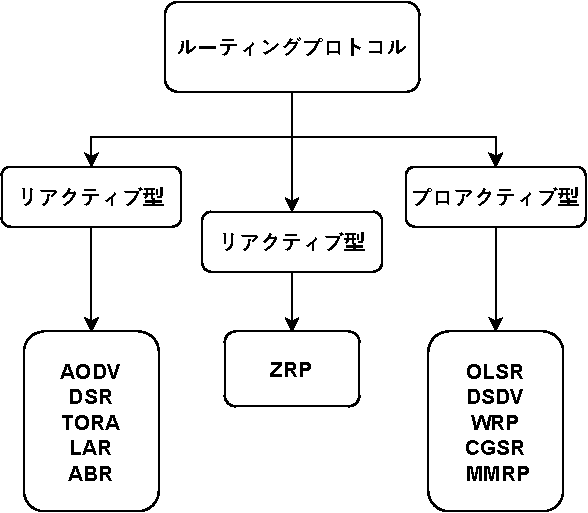
\includegraphics[width=85mm]{classification_of_routing.pdf}
  \caption{ルーティングプロトコルの分類}
  \label{routing_classification}
\end{figure}

\clearpage
\subsubsection{リアクティブ型}
あるノードが通信要求を行なった時にルーティングプロトコルに基づいて電波をフラッディングし,
近隣のノードとその場で情報のやり取り行い経路生成を行う.
通信要求がなされた時に作成されるため,実際に通信が開始されるまでにラグが発生する.

このようにする理由として,アドホックネットーワークを構築するノードのデバイスがバッテリなどで駆動することが多いため,
むやみやたらに電波をフラッディングしてしまうと,電池の消費速度が速くなってしまうからである.
加えて,ノードの移動により,ネットワークが動的に変化変化しまうため,
数分前に構築された経路表の有効性が失われる場合が多い.したがって,
通信直前に経路表を生成することで電波のフラッディング回数を減らし,駆動時間の長時間化が行われる.
それゆえに,通信開始が遅くても良い環境で用いられている.

リアクティブ型での動作イメージを図\ref{reactive}に示した.
ノードA \textasciitilde Eが図のようにある時,ノードAとEが通信を行う場合を考える.
次に,リアクティブ型での経路構築の手順を示す.

\begin{enumerate}[label=\ding{\numexpr171+\arabic*}]
  \item \label{1} ノードAが自身のIDと宛先ノードの情報を載せてフラッディングを行う.
  \item \label{2} \ref{1}の情報を受信したノードは,送信元を記録してから,宛先を確認する.
  今回の場合,宛先が違うため①と同様の情報を載せてフラッディングを行う.\\
  宛先のノードに辿り着くまで行う.
  \item \label{3} \ref{2}の情報を受信したノードEは,今回の宛先であるため,これまでの経路を逆順に辿って行き,
  発信元のノードAに経路が生成されたことを伝達し,経路表をもとに通信を行う.
\end{enumerate}

\begin{figure}[h]
  \centering
  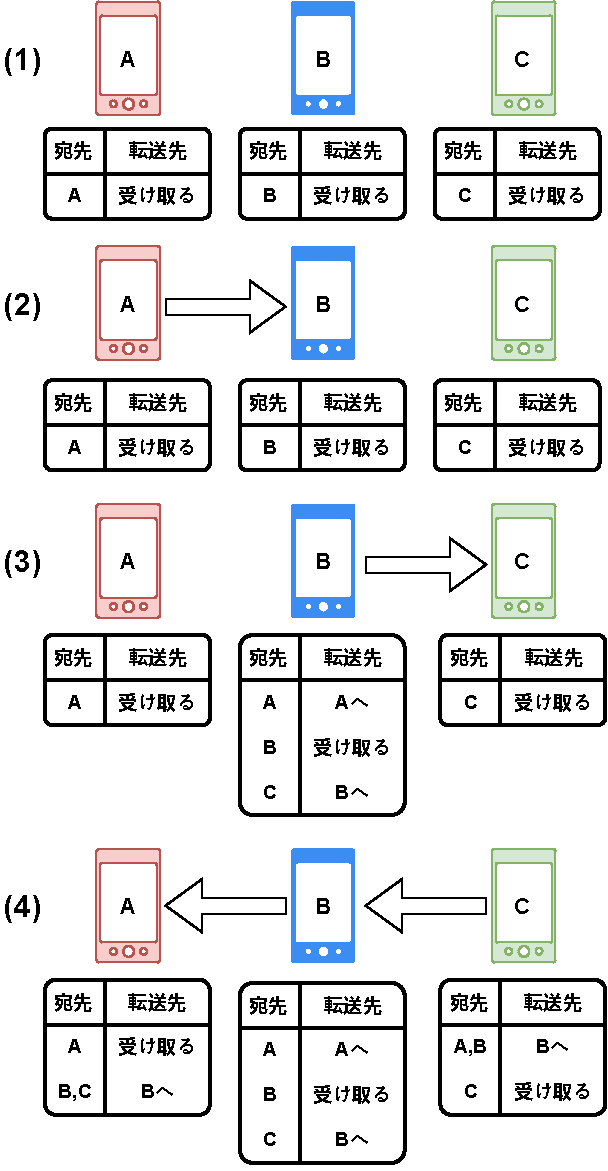
\includegraphics[width=130mm]{reactive_model.pdf}
  \caption{リアクティブ型の動作イメージ図}
  \label{reactive}
\end{figure}

ノードC, Dはノードが存在する限りフラッディングを行なってしまうため,現在の情報にフラッディングをする回数も同時に
送信し,回数が0になったら,これ以上の探索は実施しないという対策が必要となる.

代表的なプロトコルとしてAODV,DSR,TORA,LAR,ABRなどがある.次にそれぞれの特徴について概説する.

\begin{itemize}
  \item AODV(Ad hoc On-Demand Distance Vector)\cite{AODV} \\
  AODVとは,アドホックネットワークの構築と維持を望むノード間で
  動的かつ自己開始型のマルチホップルーティングを可能とするプロトコルである.
  
  AODVでは,ノードが新たな宛先への経路を要求した際に即座に経路を構築し,
  ネットワークに参加していないノードの経路情報を保持しないという特徴がある.加えて,
  ネットワークトポロジの変化に適応し,接続の断絶や変更に対して即時に対応が可能である.
  各ノードは,次ノードの情報を保持するため,接続が切れても周辺のノードにしか影響が行かないため,
  オーバーヘッドが少ない.しかし,遠くのノードの存在を知ることができないためループが発生しても
  検知ができない.そのため,フラッディングする情報の中にシーケンス番号を入れ,
  情報に有効期限を持たせループを回避する.\\
  
  \item DSR(Dynamic Source Routing)\cite{DSR} \\
  DSRとは,AODVと同様な必要時に経路を構築と維持を行う動的なプロトコルである.加えて,
  一度生成された経路を基に通信を行う,キャッシュを利用した手段もある.

  DSRでは,アドホックネットワークの経路構築と維持を行うにあたって,ルートディスカバリーと
  ルートメンテナスの2つの主要なメカニズムで構成されている.
  AODVでは,各ノードが次ホップ情報を管理しているため,オーバーヘッドは少ないが,
  DSRでは,送信元ノードが経路情報を管理するため,オーバーヘッドが大きくなってしまう.
  しかし,再度通信を行うとき,一度通信をした記録があれば即座に通信を行うことができる.
  加えて,送信元ノードが経路情報を保持しているため,同じノードを経由したとき,
  それ以上のループを行わないようすることが可能になる.\\
  
  \item TORA(Temporally-Ordered Routing Algorithm)\cite{TORA} \\
  TORAとは,動的なネットワークトポロジの変化に適応することを目的とした
  分散型ルーティングプロトコルである.

  TORAでは,ネットワークトポロジの変化に適応するために,参加したノードや
  接続が切断されたノードの通知を局所的に行い,広範囲な更新を行わないことで,
  通信のオーバーヘッドを抑え,ネットワーク規模が拡大しても対応可能になる.
  また,これまでのプロトコルでは,宛先までの単一方向の経路情報しか保持しなかったが,
  TORAでは,各ノードは隣接ノードのみの情報を保持するため,送信元に戻る選択肢がなくなり,
  ループが抑制可能になる.加えて,複数の経路表を作成することも可能となり,
  経路表の中で接続が切断されたノードが発生しても,予備の経路を使うことで通信を維持すること
  が可能となる.\\

  \item LAR(Location-Aided Routing)\cite{LAR} \\
  LARとは,ノードの地理的な位置情報を活用することで,ルーティングの探索範囲を制限し,
  通信のオーバーヘッドを削減することを目的としたプロトコルである.

  従来のリアクティブ型プロトコルでは,宛先ノードを発見するためにネットワーク全体に情報を
  フラッディングするため,不要なリクエスト情報が大量に発生し,ネットワークの帯域を圧迫していた.しかし,
  LARでは,GPS(Global Positioning System)等で各ノードの位置情報を取得し,ルート探索の際に
  情報をフラッディングするノードを限定することで帯域の圧迫を阻止することで可能となる.

  探索方法として,送信元は他ノードとの事前のやり取りで宛先ノードの大まかな位置情報を取得しており,
  経路探索を行う際に,宛先ノードの最終位置と移動速度を元に宛先ノードが存在する可能性が
  高い領域,期待領域を計算により求め,宛先ノードが移動する可能性のある範囲を推測する.
  また,フラッディングの拡散を制限するために,経路探索の範囲をリクエスト領域を設定する.
  これは,送信元と期待領域が含まれるように設定される.

  これらの設定が完了した後,送信元がリクエスト領域に情報をフラッディングし,
  領域内にいるノードのみが中継行う.そして,宛先に到達したら,送信元にこれまでの
  経路を送信し,最適な経路を構築させる.また,宛先に到達しなかった場合,
  リクエスト領域の範囲を拡大させ再度経路探索を行う.

  これにより,過剰なフラッディングを抑制かつ経路構築の高速化が可能となる.しかし,
  全てのノードがGPSを搭載している必要がある.また,リクエスト領域を正しく設定を行わないと,
  再探索が発生するため,通常より長い遅延が発生する可能性がある.\\

  \item ABR(Associativity-Based Routing)\cite{ABR} \\
  ABRとは,アソシアティビティ(持続の安定性)の概念を活用しており,長時間接続が維持される
  ノードを優先的に利用することで,頻繁な経路の再構築を抑制するプロトコルである.

  ABRでは,アソシアティビティティック(Associativity Ticks),
  いわゆる接続安定度と呼ばれる数値が定義されている.また,このプロトコルでは,
  ノードが移動している移動期間とノードが静止している安定期間と呼ばれる二つの状態が定義されている.
  そして,この二つの期間の境界を示す閾値をアソシアティビティ閾値と定義された.
  
  ノードが移動中の場合,ティックは低い値となり,静止している場合,高い値を示す.
  ティックの数値がアソシアティビティ閾値を超えたとき,そのノードは安定しているとみなされ,
  通信時の中継ノードとして利用される.このため,ノードは定期的に隣接ノードとやり取りを行い,
  隣接ノードのティックを更新する.

  これにより,不要な経路を保持しないため,オーバーヘッドの削減やその経路の信頼性が
  向上する.

\end{itemize}


\clearpage
\subsubsection{プロアクティブ型}
リアクティブ型では通信要求が発生してから経路表が作成されるのに対し,プロアクティブ型では近隣のノードと周期的に情報のやり取りを行い,
通信要求が発生したらすぐに通信を開始することができる.しかし,リアクティブ型と比べ頻繁に情報のやり取りを行うため,電池の消費が早い.
常に新鮮な経路表を保持しているためノードの入れ替わりが激しい環境では有効的である.

以下にリアクティブ型での動作イメージを図\ref{proactive}に示した.各ノードは常に近隣のノードと情報をやり取りしているため,
通信の開始が早く,また,近隣のノードが接続が不可能になったとしても,すぐに新たな経路を生成することが可能であり安定した通信を行うことができる.
\begin{figure}[h]
  \centering
  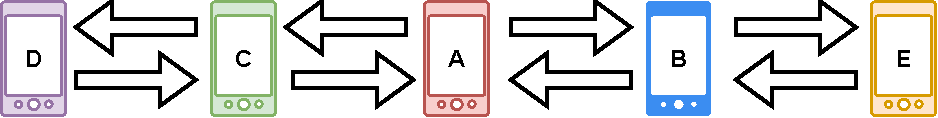
\includegraphics[width=130mm]{proactive_model.pdf}
  \caption{プロアクティブ型の動作イメージ図}
  \label{proactive}
\end{figure}

代表的なプロトコルとしてOLSR,DSDV,WRP,CGSR,MMRPなどがある.
次にそれぞれの特徴について概説する.

\begin{itemize}
  \item OLSR(Optimized Link State Routing)\cite{OLSR}\\
  OLSRとは,定期的に行われる通信で得たネットワーク全体のトポロジ情報を元に
  最適経路を求めるプロトコルである.経路を求める方法として,有線LANで使用される
  OSPF(Open Shortest Path First)で計算される.

  このプロトコルでは,ネットワークトポロジ情報の更新時,効率的に行うために
  MPR(MultiPoint Relay)集合と呼ばれるものを用いるのが特徴である.
  
  通常のフラッディングの場合,初めて情報を受信したノードは必ず一度は近隣ノードに
  情報をフラッディングする.しかし,近隣ノードの中にすでに同じ情報を受け取っている
  ノードがいる可能性があるため,無駄な通信が発生する.そして,これを防ぐために
  MPR集合を用いて中継ノードを決定し,効率的な情報の伝搬を行う.
  
  \begin{itemize}
    \item MPR集合とは,1ホップ内の隣接ノードと2ホップ内の隣接ノードがある場合,
    1ホップ内の隣接ノードの中から2ホップ内の隣接ノードをカバーできる1ホップ内のノードを
    MPRノードとして選定し,MPRノード以外はフラッディングをしない.
    そして,3ホップ,4ホップ,\dots,と数が増えても同様にMPRノードを選択を行う.
    このノードの集合をMPR集合という.\\
  \end{itemize}

  \item DSDV(Destination-Sequenced Distance-Vector)\cite{DSDV}\\
  DSDVとは,リアクティブ型のAODVと同様なアルゴリズムであり,
  シーケンス番号でループを回避するが,近隣ノードと定期的に通信を行うため,
  ノードの接続が切断された場合でも,予備の経路を構築でき,
  AODVより安定した通信を実施が可能である.

  しかし,ネットワークトポロジの規模大きいまたは変化が激しい環境では,
  トポロジ更新によるオーバーヘッドが大きくなり,経路更新の効率が低下してしまう.\\

  \item WRP(Wireless Routing Protocol)\cite{WRP}\\
  WRPとは,DSDVプロトコルの問題を改善し,ループを回避しつつ,より効率的な経路更新を
  行うプロトコルである.

  WRPでは,距離テーブル,ルーティングテーブル,リンクコストテーブル,メッセージ再送テーブルの
  4つのテーブルを各ノードが管理し,ループを回避し,効率的な経路構築を行う.次に,各テーブルの
  機能を示す.
  \begin{itemize}
    \item 距離テーブル:各隣接ノードが把握している経路情報を記録.最適な経路を構築する際に使用.
    \item ルーティングテーブル:実際に使用する経路情報のホップ数などを記録.
    \item リンクコストテーブル:隣接ノードとの品質,安定度を記録.
    \item メッセージ再送テーブル:経路更新メッセージを管理.更新メッセージが未応答のノードに対して
    確認メッセージの再送を行う.\\
  \end{itemize}

  \item CGSR(Cluster-head Gateway Switch Routing)\cite{CGSR}\\
  CGSRとは,クラスタと呼ばれるノードの集合を動的に生成し,クラスタ間で別チャネルを用いて
  通信を行うことで,情報の衝突を防ぐプロトコルである.

  CGSRでは,クラスタ内でノードがヘッダ,メンバ,ゲートウェイのどれかに割り当てらる.
  \begin{itemize}
    \item クラスタヘッダ:クラスタ間の通信を管理するノード
    \item クラスタメンバ:一つのクラスタヘッドに属するノード.
    他ノードと通信する際,クラスタヘッダを経由して通信を行う.
    \item クラスタゲートウェイ:複数のクラスタに所属しているノード.
    クラスタ間の通信の際,チャネルを変更する中継処理の役割を持つ.
  \end{itemize}

  このプロトコルでは,クラスタ単位でノードを管理するためネットワークの規模が拡大しても
  管理他のに比べ,容易である.しかし,クラスタヘッダが通信時に経由されるため,他ノードと比較して
  電力を多く消費する.その結果,ネットワーク全体の寿命が短い.\\

  \item MMRP(Mobile Mesh Routing Protocol)\cite{MMRP}\\
  MMRPとは,ネットワークトポロジをメッシュ型で構築するプロトコルである.

  MMRPでは,ノードが移動により接続が切断された場合,切断されたノード間の経路を他ノードを
  経由するように切り替るため,通信経路を確立でき通信が安定する.
  しかし,ノードが移動中での通信は頻繁に接続するノードが変化するため,移動ノードの通信は
  安定しない.

\end{itemize}

\subsubsection{ハイブリッド型}
リアクティブ型とプロアクティブ型の長所を組み合わせたプロトコルである.
代表的なプロトコルとしてZRP(Zone Routing Protocol)\cite{1574231874891177344}がある.

図\ref{hybrid_model}にZRPの動作イメージを示す.ZRPでは,ゾーンと呼ばれる範囲で使用するプロトコルを
分ける.この図では,ノードAを中心としてホップ数を1とした場合のゾーン半径を示す.そして,ゾーン内に
存在するノードはプロアクティブ型でネットワークを構築する.また,ゾーン外のノードには,
リアクティブ型で通信要求が発生した時に経路構築を行う.

メリットとして,ゾーン内では短距離通信の遅延が最小化され,ゾーン外では不要な情報のやり取りを減らすことが可能となる.
また,ネットワークが大規模になったとしても全ての経路情報を保持しなくて良いため効率的に運用することが可能である.
しかし,デメリットとして,ゾーン半径の設定が困難なことである.
ゾーン半径が小さい場合,遠距離通信が頻繁に発生する.また,
ゾーン半径が大きい場合,ゾーン内に存在するノードが多数になり計算コストとメモリ消費が増大する.

\begin{figure}[h]
  \centering
  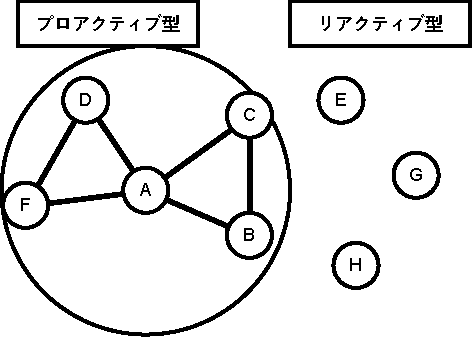
\includegraphics[width=70mm]{hybrid_model.pdf}
  \caption{ハイブリッド型の動作イメージ図}
  \label{hybrid_model}
\end{figure}

% \clearpage
\subsection{アドホックネットワークの技術的課題}
\ref{about_ad-hoc}節で述べた課題のほかに,隠れ端末問題とさらし端末問題があり,
これらがアドホックネットワークが一般的に普及されていない原因の一つとも言える\cite{松井_進2012KJ00008330022}.
次項にそれぞれの問題について説明する.
\subsubsection{隠れ端末問題}
図\ref{hidden_problem}に隠れ端末問題を表した図を示す.図\ref{hidden_problem}では,
スマートフォンがノード,その周りにある円がノードからの通信距離を表している.
ノードBの円は見やすさの都合上省略している.

隠れ端末問題とは,ノードAとCがノードBに接続を行うとき,ノードA,Cは互いに通信可能距離外にあるため
互いの存在が隠れてしまい,ノードBが誰とも通信をしてないと判断してしまう.
そして,ノードA,Cが同時にデータをノードBに送信した場合,電波干渉やデータの衝突する問題が発生がある.

この問題により通信制御のスループット(処理能力)の低下が発生し,通信に遅延が生じる.
\begin{figure}[h]
  \centering
  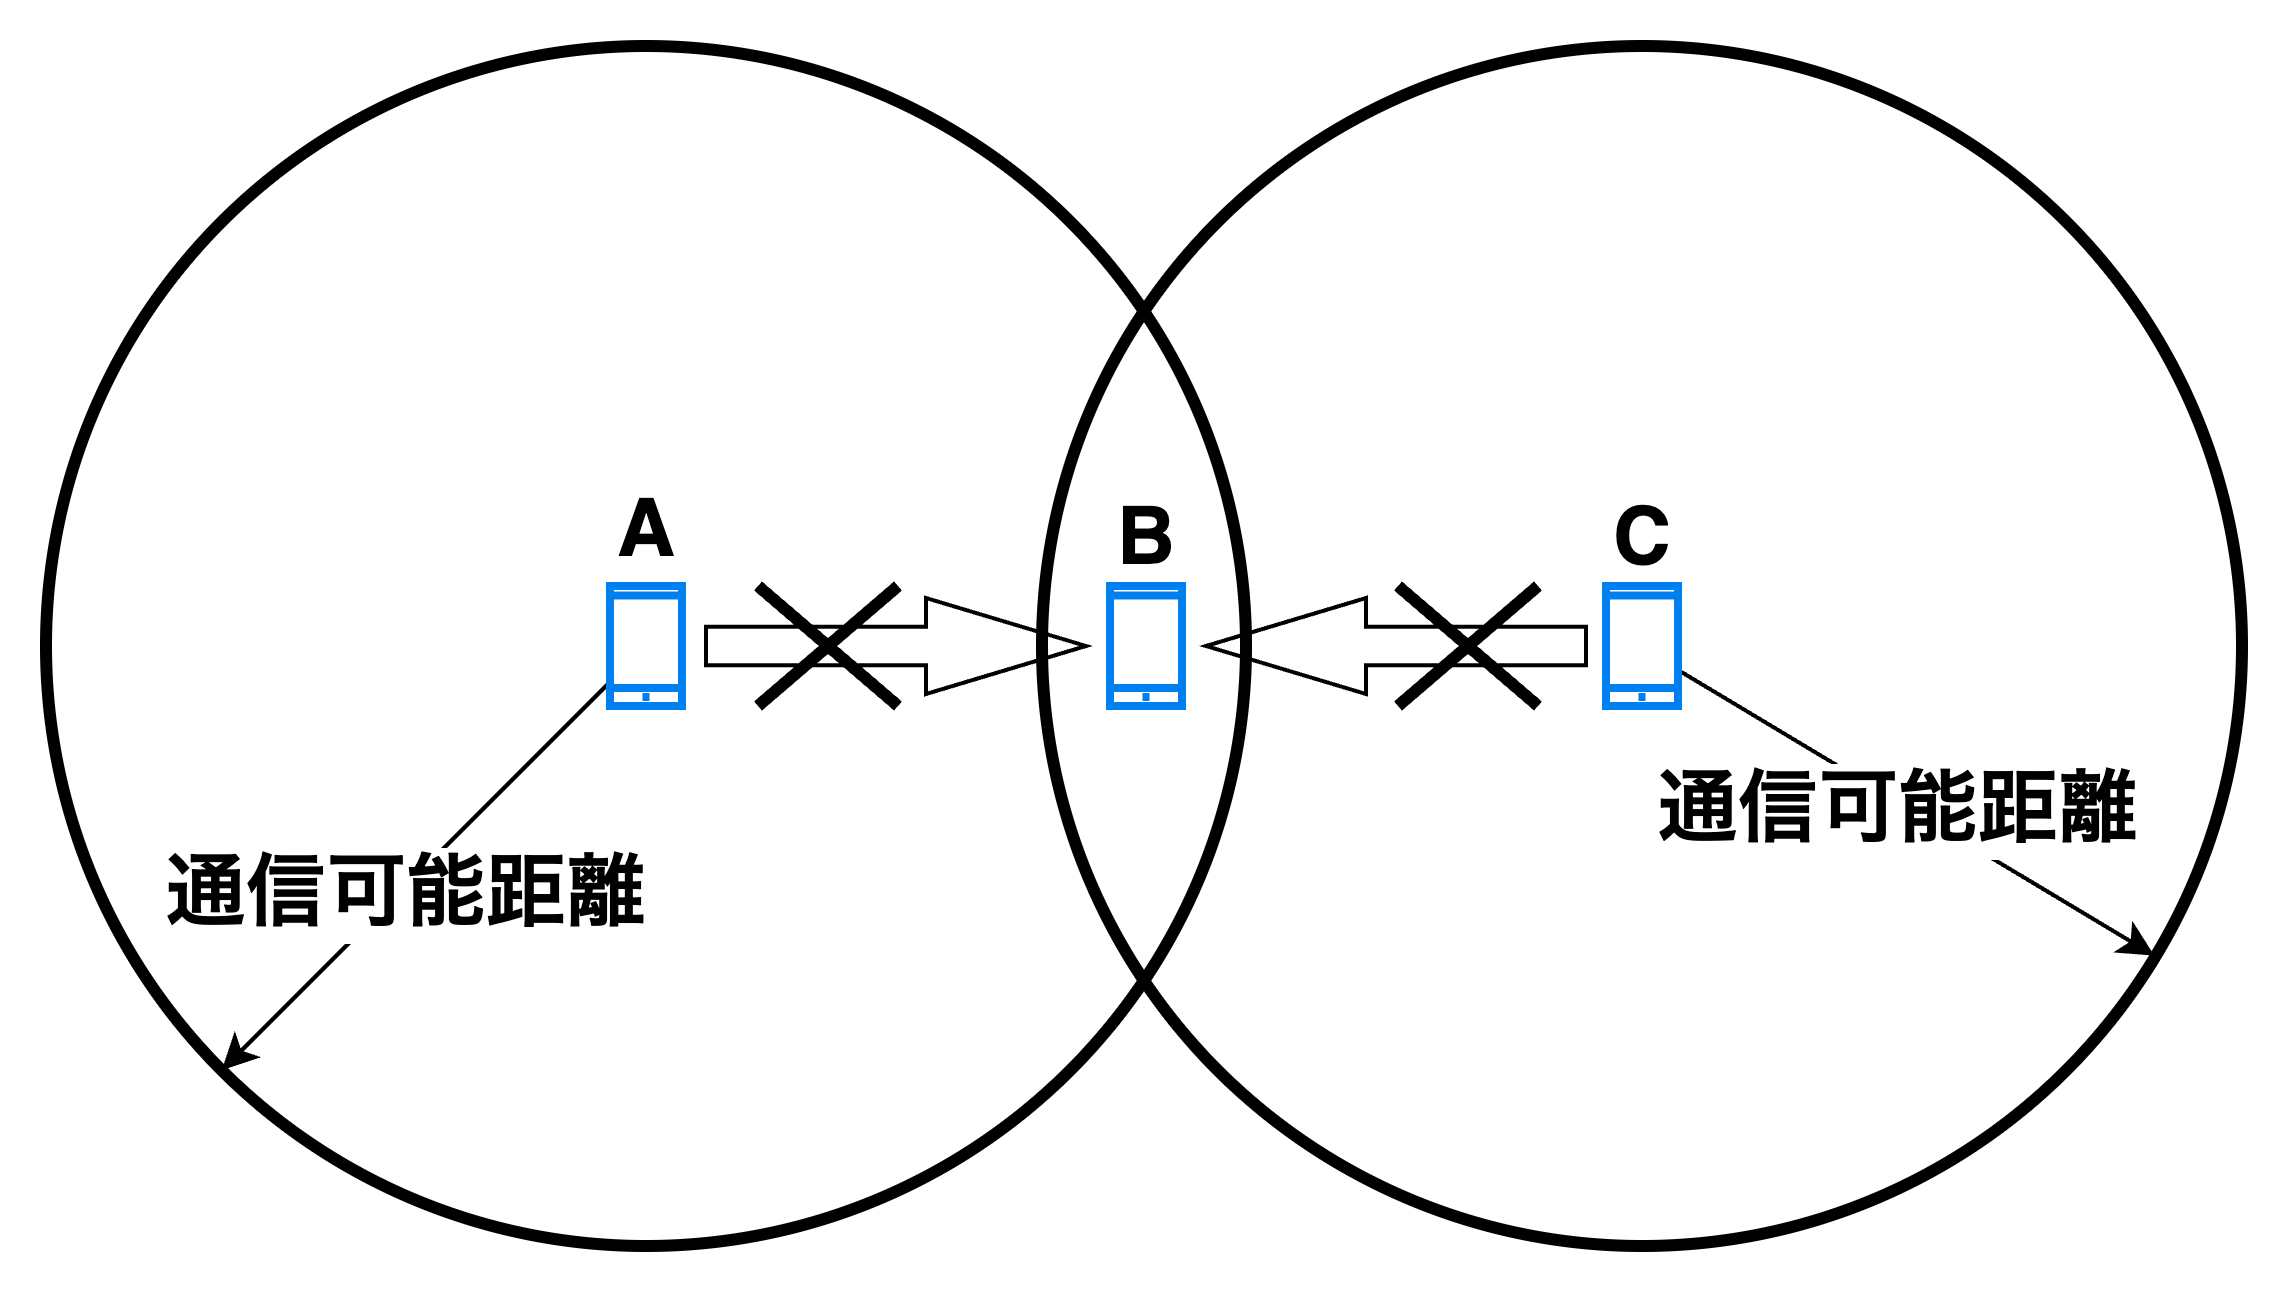
\includegraphics[width=80mm]{hidden_terminal_problem.png}
  \caption{隠れ端末問題}
  \label{hidden_problem}
\end{figure}

\subsubsection{さらし端末問題}
図\ref{exposed_problem}にさらし端末問題の図を示す.
図\ref{exposed_problem}で表されているスマートフォンや円は隠れ端末の場合と同様の意味である.

さらし端末問題とは,他ノードからの過剰な通信抑制による伝送速度や通信品質の低下が発生する
問題である.図のように,ノードAとDが通信を行い,ノードBとCが通信を行う場合を考える.
ノードAとBが互いに通信可能範囲内にいるとき,お互い別のノードと通信しているのにも
関わらず, お互いに通信を開始しないように通信抑制が頻繁に行われ,結果的に伝送速度が低下してしまう.

\begin{figure}[h]
  \centering
  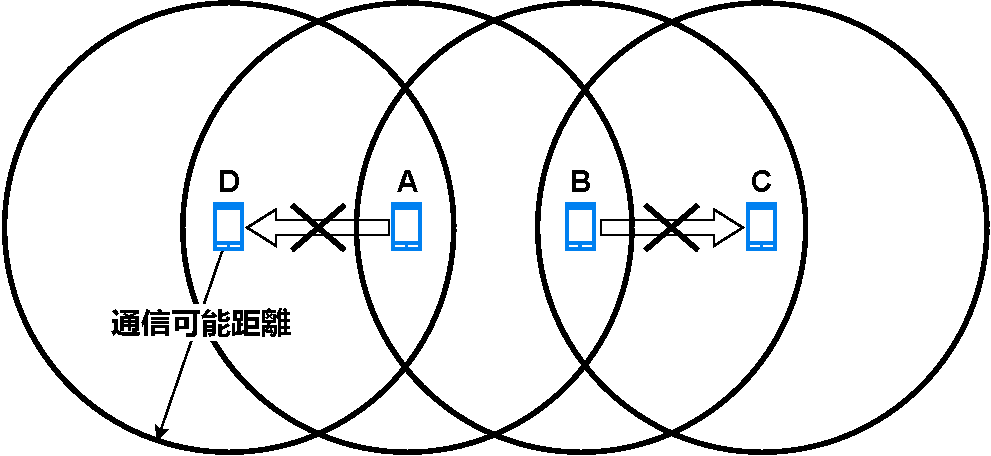
\includegraphics[width=80mm]{Exposed_terminal_problem.pdf}
  \caption{さらし端末問題}
  \label{exposed_problem}
\end{figure}

% \clearpage
\subsection{Bluetooth}
Bluetoothとは,デジダル機器用の近距離無線通信規格の一つであり,数メートルから数十メートル程度での距離間で電波を用いて簡易的な情報のやり取りを行う.
加えて,免許を必要としない2.4GHzの周波数帯を使用するためPCのマウスやキーボード,ワイヤレスイヤホン,スマートウォッチなど生活の身近に使用されている.
IEEEの規格名はIEEE802.15.1である.

1994年,スウェーデンのEricsson社が近距離無線通信規格の開発をはじめ,
1998年にPromoter5社(Ericsson,Intel,IBM,Nokia,東芝)によりBluetooth SIG(Special Interest Group)
が設立され,Bluetothの規格策定が行われている.そして,現在まで公開されている仕様として,
Bluetooth ClassicとBluetooth Low Energy(LE)の2種類に分けることができる.
表\ref{Bluetooth_characteristics}にそれぞれの特徴を示した.

\begin{table}[h]
  \centering
  \caption{Bluetooth ClassicとBLEの特徴\cite{Bluetooth_official}}
  \begin{tabular}{c|c|c}
    \specialrule{1.5pt}{0pt}{0pt} % 上端の太線(1.5pt)
       & Bluetooth Classic & BLE \\
      \hline
      周波数帯 & \multicolumn{2}{c}{2.4GHz (2.402 \textasciitilde 2.480GHz)} \\
      \hline
      チャネル利用 & \multicolumn{2}{c}{周波数ホッピングスペクトラム拡散 (FHSS)} \\
      \hline
      チャネル数 & 1MHz間隔で79チャネル & \makecell{2MHz間隔で40チャネル\\(3つはアドバタイジング用チャネル)} \\
      \hline
      転送速度 & 3, 2, 1 Mbps &  2, 1 Mbps,500, 125 kbps \\
      \hline
      同時接続台数 & 最大7台 & 仕様上無限 \\
      \hline
      消費電力 & 1W & 0.01W \textasciitilde 0.5W \\
      \hline
      通信トポロジ & スター型 & スター型,メッシュ型 \\
      \hline
      主な用途 & マウス,イヤホンなど & IoTセンサ,スマートウォッチなど \\
      \specialrule{1.5pt}{0pt}{0pt} % 上端の太線(1.5pt)
  \end{tabular}
  \label{Bluetooth_characteristics}
\end{table}

\subsubsection{Bluetooth Classic}
Bluetooth Classicとは,1997年に一般公開されたBluetooth 1.0から3.0までのバージョンを指す.

デバイスには,接続要求を行う親機(Master)と接続要求を受ける子機(Slave)の2種類ある.Masterはいわゆるスマートフォン,
Slaveはワイヤレスイヤホン等のガジェットに相当するものである.この時,Masterは同時に最大7台のSlaveと接続が可能.
また,Bluetoothで位置検出を行う研究が行われている\cite{勝野_恭治2002}.

通信距離はClass1\textasciitilde3のように電波強度で分類され表\ref{Classic_connecting_distance}のようになっている.

\begin{table}[h]
  \centering
  \caption{Bluetooth Classicの場合\cite{東芝情報システム株式会社}}
  \begin{tabular}{c|l}
    \specialrule{1.5pt}{0pt}{0pt} % 上端の太線(1.5pt)
      Class 1 & 最大 100m (4dBm超 \textasciitilde 20dBm) \\
      \hline
      Class 2 & 最大 10m (0dBm超 \textasciitilde 4dBm) \\
      \hline
      Class 3 & 最大 1m (0dBm) \\
      \specialrule{1.5pt}{0pt}{0pt} % 上端の太線(1.5pt)
  \end{tabular}
  \label{Classic_connecting_distance}
\end{table}

\subsubsection{Bluetooth LE}
Bluetooth LEとは,2009年のに公開されたBluetooth 4.0以上のバージョンを指し,
このバージョンから低消費電力デバイス向けに,より省電力に特化した機能が追加された.

Bluetooth LEのデバイスでは,親機をCentral,子機をPeripheralと呼称が変わる.先ほどとデバイスの意味合いは同じだが,
Centralが同時に接続できるPeripheralの数は仕様上無限という違いがある.しかし,Bluetoothチップ等の
デバイスに依存する.
また,Bluetooth 5からは多 対 多のメッシュネットワークを構築できるようになり,アドホックネットワーク利用への
期待が高まっている.本研究では,災害時いつインフラが回復するか不明の状況を想定しているため,
長時間駆動に特化したBluetooth LEを搭載したノードを用いた場合でシミュレーションを行った.

通信距離はデータ転送速度で異なり,表\ref{BLE_connecting_distance}のようになっている.

\begin{table}[h]
  \centering
  \caption{BLE(最大出力が20dBm)の場合\cite{東芝情報システム株式会社}}
  \begin{tabular}{c|c}
    \specialrule{1.5pt}{0pt}{0pt} % 上端の太線(1.5pt)
    2Mbps & 最大 100m \\
    \hline
    1Mbps & 最大 100m \\
    \hline
    125kbps & 最大 400m \\
    \specialrule{1.5pt}{0pt}{0pt} % 上端の太線(1.5pt)
  \end{tabular}
  \label{BLE_connecting_distance}
\end{table}

% %---先行研究---------------------------------------------------------------------------------------
% \clearpage
% \section{先行研究}

%---提案手法---------------------------------------------------------------------------------------
\clearpage
\section{提案手法} \label{提案手法}
本研究では,人口密度に基づくアドホックネットワークの構築方法を提案する.

まず,アドホックネットワークを用いる場面として,地震等の大規模災害による基地局の損壊や停電等により
ネットワークにアクセスができない場面だと考えられる.
また,通信インフラが機能しない状況では,基地局の停電が復旧するまでの間,生き残っている基地局にアクセスが集中することで回線が混雑し,
家族や知人の安否確認ができなくなり,救助を必要としている人の声が救急隊まで届かない.加えて,ネットワークにアクセス
ができないため,現在の被災状況を知ることができないなど,被災者の精神的負担が大きくなってしまう.
この事態を避けるために,被災地域限定でアドホックネットワークを通信インフラが復旧するまでの間利用することで,
現在の被災状況や避難場所,安否確認等を行え,被害の拡大防止や被災者の不安を和らげることが可能になると考えられる.

しかし,先ほどのような被災状況でアドホックネットワークを構築する際,重要になってくるのがノードの密度である.
なぜなら,ノードの通信範囲内にノードが存在しなければネットワークを拡大することができないからだ.
その上,自然災害は予測不能であり,被災地の通信環境は地域ごとに大きく異なる.特に,
人口密度が低い地域の場合,ノード数が少なく,間隔も広がるためアドホックネットワークを構築するのが困難になる.
これを解決するために,初めに各都道府県に対して今回作成したシミュレーションを実行し,本研究内での
人口密度が高い,低い地域を選定する.この結果を元に,人口密度が低い地域に対して,公共物である電柱にノードを追加し
た場合のシミュレーションを実施し,その有効性について検証する.

\subsection{シミュレーション仕様}
シミュレーションで使用するノードは,消費電力が少ないBluetooth LEとし,
その接続目安距離である30mを最大通信距離とした.
また,実施する範囲は1km四方の平面上で,その範囲内にノードをランダムで生成する.生成するノード数は,
2024年10月1日現在の各都道府県の人口密度\cite{人口密度}にスマートフォンの所有率88.6\%\cite{スマホ保有率}を乗じた数とした.
表\ref{table:人口密度}に各都道府県の人口密度とノード数を左から降順に示す.

\begin{table}[h]
  \centering
  \caption{各都道府県の人口密度\cite{人口密度}}
  \begin{tabular}{l|c|c||l|c|c||l|c|c}
    \specialrule{1.5pt}{0pt}{0pt} % 上端の太線(1.5pt)
    地名 & 人口密度 & ノード数 & 地名 & 人口密度 & ノード数 & 地名 & 人口密度 & ノード数 \\
    \hline
    東京都 & 6451 & 5716 & 広島県 & 320 & 284 & 大分県 & 171 & 152 \\
    \hline
    大阪府 & 4603 & 4078 & 宮城県 & 309 & 274 & 新潟県 & 167 & 148 \\
    \hline
    神奈川県 & 3817 & 3382 & 長崎県 & 303 & 268 & 鹿児島県 & 167 & 148 \\
    \hline
    埼玉県 & 1930 & 1710 & 群馬県 & 297 & 263 & 徳島県 & 165 & 146 \\
    \hline
    愛知県 & 1443 & 1278 & 三重県 & 296 & 262 & 鳥取県 & 151 & 134 \\
    \hline
    千葉県 & 1217 & 1078 & 栃木県 & 294 & 260 & 長野県 & 147 & 130 \\
    \hline
    福岡県 & 1022 & 905 & 石川県 & 262 & 232 & 宮崎県 & 133 & 118 \\
    \hline
    沖縄県 & 643 & 570 & 岡山県 & 257 & 228 & 福島県 & 126 & 112 \\
    \hline
    兵庫県 & 635 & 563 & 富山県 & 234 & 207 & 青森県 & 121 & 107 \\
    \hline
    京都府 & 547 & 485 & 熊本県 & 229 & 203 & 山形県 & 108 & 96 \\
    \hline
    香川県 & 489 & 433 & 愛媛県 & 225 & 199 & 島根県 & 96 & 85 \\
    \hline
    茨城県 & 461 & 408 & 山口県 & 209 & 185 & 高知県 & 92 & 82 \\
    \hline
    静岡県 & 453 & 401 & 和歌山県 & 186 & 165 & 秋田県 & 77 & 68 \\
    \hline
    滋賀県 & 349 & 309 & 岐阜県 & 180 & 159 & 岩手県 & 75 & 66 \\
    \hline
    奈良県 & 348 & 308 & 山梨県 & 177 & 157 & 北海道 & 64 & 57 \\
    \hline
    佐賀県 & 322 & 286 & 福井県 & 176 & 156 & & & \\
    \specialrule{1.5pt}{0pt}{0pt} % 上端の太線(1.5pt)
  \end{tabular}
  \label{table:人口密度}
\end{table}

% アドホックネットワークを構築する際に,通信可能距離内に複数のノードが存在するとき,どのノードと接続をして良いかわからない.
% また,安価なノード(例として,ESP32等のマイコン)で接続を行う場合,メモリ数が限られているため,複雑な命令や経路情報を多く保持することができない.
% そこで,簡易的な命令,かつ,広範囲にネットワークを構築できる方法として,周辺ノードの人口密度に基づく
% 経路構築方法を提案する.
% アドホックネットワークを利用する状況として,自然災害等によるネットワーク障害が発生した時に,周辺の
% 情報を得るために利用すると考えられる.そのため,ノードに求められる条件として,通信が安定して
% 行えるかつ,ノードの駆動時間が長時間である.

% 本研究では,主に人口密度が高い地域と低い地域の場合でアドホックネットワークを構築する際に必要となる条件を
% シミュレーションを通して確認をした.また,アドホックネットワークを構築できない地域に対して公共構造物にノードを増加させる
% ことで構築が可能になるかの検証を行った.次節にシミュレーションの想定環境,ここでの人口密度が高い,低い地域の定義を
% ネットワークが構築可能かどうかで分けていく.

% ・どのような環境下でシミュレーションを行うかの動機説明\\
% ・それを克服するにはどうすればいいのか\\
% ・シミュレーションの条件\\
% ・シミュレーションの実行例\\
% ・どの地域に対して行ったか\\
% ・人口密度が高い地域と低い地域の選定方法\\
% ・人口密度が低い地域でも安定してアドホックネットワークを構築するにはどうするかの提案\\

\clearpage
\subsubsection{アルゴリズム} \label{algorithm}
ここでは,埼玉県の人口密度1930人/$\mathrm{km^2}$,ノード数1710個を用いてアルゴリズムの説明を行う.

前提として,全てのノードが周辺にいるノードと接続するようにアドホックネットワークを
構築してしまうと,経路全体の複雑化や冗長化になり,通信速度や品質が低下してしまう.
この課題を解決するために経路を単純化する必要があると考えた,
そこで,ノードの接続条件を次のように定めた.


\begin{enumerate}[label=\ding{\numexpr171+\arabic*}]
  \item \label{2-1} 情報を送信するノード(以下,上流ノードと呼ぶ)が情報を受け取るノード(以下,下流ノードと呼ぶ)に対してhelloメッセージと自身のMACアドレスをフラッディングする.
  \item \label{2-2} 受信した下流ノードはreplyメッセージと自身のMACアドレスを上流ノードに返す.但し,他ノードと接続済みの下流ノードは上流ノードのhelloメッセージを無視する.
  \item \label{2-3} 上流ノードはhelloメッセージの返信数で下流ノードの数を認識する.
  \item \label{2-4} 下流ノード数が閾値$X$より大きいなら下流ノードの中からランダムで1つ選択し,そうでないならランダムで2つ,下流ノード数が2以下ならそのノードと接続する.
  \[
    \text{接続ノード数} = 
    \begin{cases} 
    \text{下流ノード数} > X \rightarrow 1, \\
    \text{下流ノード数} \leq X \rightarrow 2, \\
    \text{下流ノード数}  \leq 2 \rightarrow \text{下流ノード数}
    \end{cases}
  \]
\end{enumerate}
$X$はノード密度の閾値である.$X$を大きくすると接続ノード数が増加し,
小さくすると接続ノード数が減少する.

次に、先ほどの条件を閾値$X = 5$としてシミュレーションした場合について、より具体的に説明を行う。
\begin{enumerate}[label=\textbf{(\arabic*)}]
  \item 初期状態 \\
        図\ref{figure:first_step}にシミュレーションの初期状態を示す.

        この図において,黄色の点はノード未接続ノード,赤色の点はスタートノードおよびターゲットノードを示している.
        また,中心に最も近い赤色のノードをスタートノード,中心から最も遠い位置にある赤色のノードをターゲットノードとし,
        接続の成功を判断する指標とした.
        
        \begin{figure}[h]
          \centering
          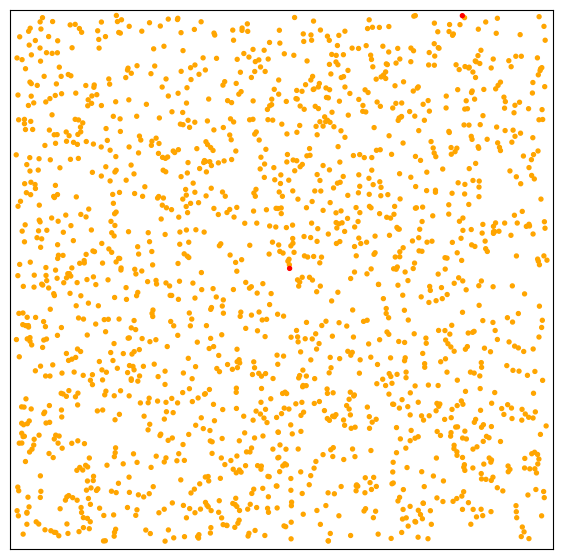
\includegraphics[width=100mm]{1_step.png}
          \caption{初期状態図}
          \label{figure:first_step}
        \end{figure}
  \clearpage
  \item 接続可能ノードの探索 \label{探索} \\
        図\ref{figure:first_step}のスタートノードに注目し拡大した図を図\ref{figure:second_step}に示す.
        この図で青の円は,スタートノードを中心とした通信可能範囲を示しており,\ref{2-1}のように,
        通信可能範囲内に存在するノードへ情報を送信している状態である.
        また,ノードの接続条件において,上流ノードはスタートノードに相当する.
        
        \indent シミュレーションでは,\ref{2-2},\ref{2-3}の過程をこの時に同時に行っており,上流ノードは接続可能な下流ノードの
        数を保持している.

        \begin{figure}[h]
          \centering
          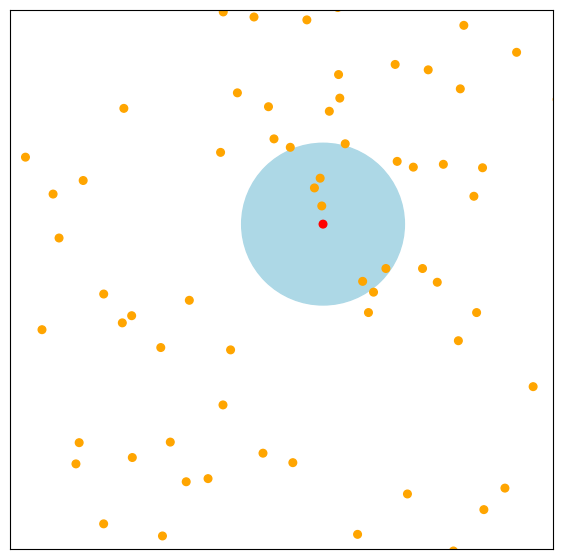
\includegraphics[width=80mm]{2_step.png}
          \caption{接続可能ノードの探索図}
          \label{figure:second_step}
        \end{figure}
  \item ノード接続 \\
        図\ref{figure:third_step}に上流ノードが下流ノードとランダムに接続した様子を示す.
        今回の場合では,下流ノード数が5であるため,接続ノード数は2となる.そして,接続されたノードは
        青色の点で示した.

        次に,今回選ばれたノードが上流ノードとなり,\ref{探索}と同様に隣接ノードを探索し,
        未接続ノードがいなくなるまで行う.

        \begin{figure}[h]
          \centering
          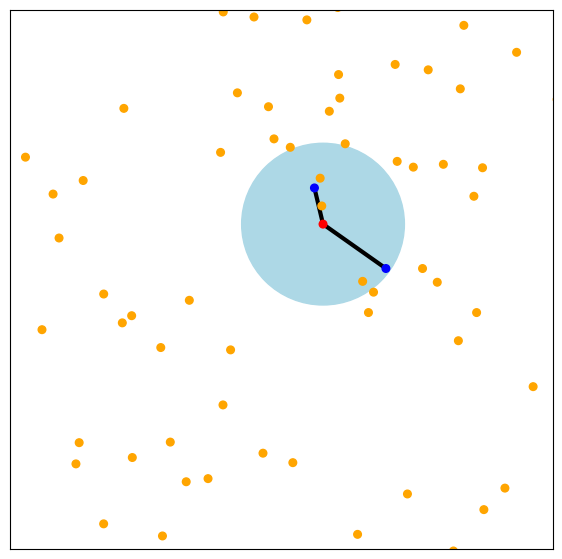
\includegraphics[width=80mm]{3_step.png}
          \caption{ノード接続図}
          \label{figure:third_step}
        \end{figure}
  \clearpage
  \item 経路完成 \\
        図\ref{figure:fourth_step}に探索が終了した際の図を示す.
        赤線はスタートノードからターゲットノードまでの経路を示している.
        結果では,青ノードをノードの総数で割り,通信成功割合を元に
        人口密度の高低を定める.通信成功割合の計算式を次に示す.
        \[
          \text{通信成功割合} [\%] = \frac{\text{接続成功ノード数}}{\text{ノード総数}} \times 100 \quad \text{(1)}
        \]

        \begin{figure}[h]
          \centering
          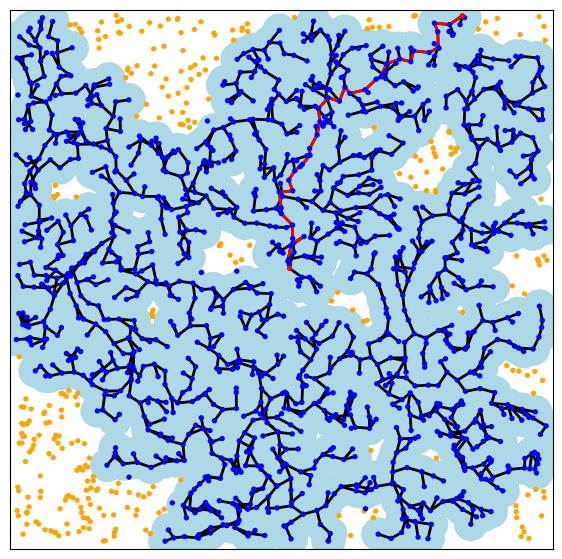
\includegraphics[width=100mm]{4_step.png}
          \caption{経路完成図}
          \label{figure:fourth_step}
        \end{figure}

\end{enumerate}

\subsubsection{人口密度が低い場合}
\ref{algorithm}項で述べたアルゴリズムでは、人口密度が低い地域ではノード間の距離が広がり、
通信可能範囲内に他のノードが存在しないため、人口密度が高い地域でのみ機能することが考えられる.
そこで、人口密度が低い地域においても通信が可能となるよう、公共物などにノードを設置し、
ノード密度を増加させることで、人口密度が高い地域と類似した環境を構築することとした。
特に、設置対象としては、移動せずかつ一定の間隔で配置される構造物が、
ルーティングの設計や実装の観点から有利である。この要件を満たすものとして、
本研究では電柱へのノード設置を想定した。
本シミュレーションでは、電柱間の距離を50mとし\cite{電柱設置間隔}、電柱間の通信は無線LAN等を用いた
直接通信が可能であると仮定する。ただし、ネットワークはメッシュ型ではなく1体1の通信を考える.

図xに,福島県の人口密度126人/$\mathrm{km^2}$,ノード数112個の条件で電柱を追加した場合の
シミュレーション結果を示す.
\begin{enumerate}[label=\textbf{(\arabic*)}]
  \item 初期状態 \\
  図\ref{figure:福島_1_step}に電柱を追加した場合の初期状態を示す.赤色と黄色の点の意味は
  先ほどと同様である.今回新たに追加された緑色の点は電柱に設置されたノード(以下,電柱ノードと呼ぶ)を示している.
  加えて,電柱間は直接通信を行えることを示すためにピンク色の線で,接続されている電柱ノードを
  示した.

  経路構築方法は\ref{algorithm}項と同様に行う.
  \clearpage
  \begin{figure}[h]
    \centering
    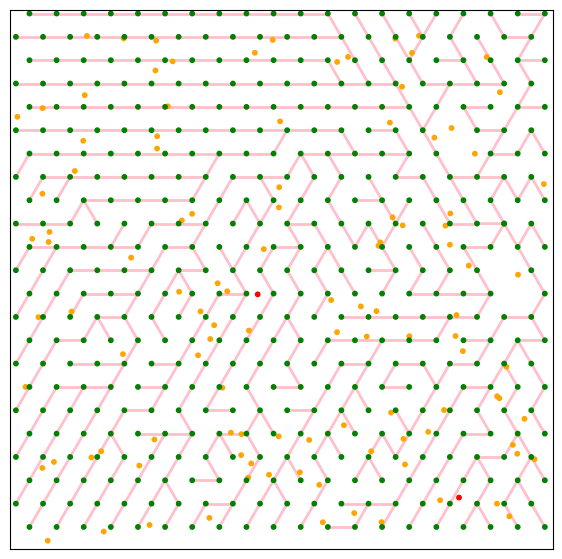
\includegraphics[width=90mm]{福島_1_step.png}
    \caption{電柱にノードを追加した場合の初期状態図}
    \label{figure:福島_1_step}
  \end{figure}

  \item 経路完成 \\
  \begin{figure}[h]
    \centering
    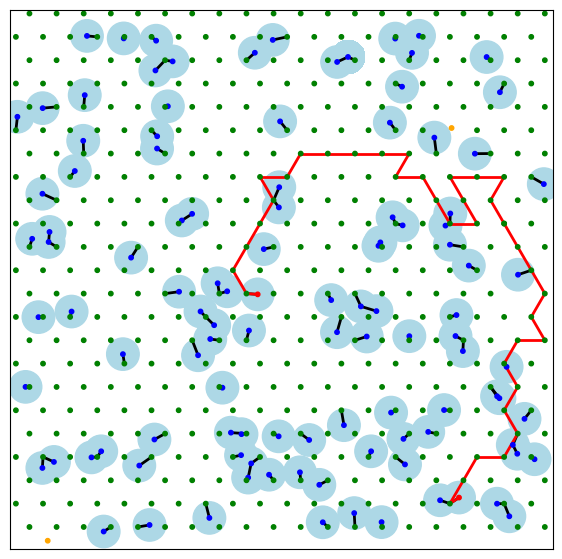
\includegraphics[width=90mm]{福島_2_step.png}
    \caption{電柱にノードを追加した場合の経路完成図}
    \label{figure:福島_2_step}
  \end{figure}
\end{enumerate}

%---結果---------------------------------------------------------------------------------------
\clearpage
\section{結果}
本研究内での,人口密度の高低をシミュレーションを通して定義する.
\ref{提案手法}章の提案手法を元に全ての都道府県のに対して閾値$X = 5$の条件で10回シミュレーションを行い,
その平均を図\ref{figure:各都道府県の通信成功割合}のグラフに示す.

\begin{figure}[h]
  \centering
  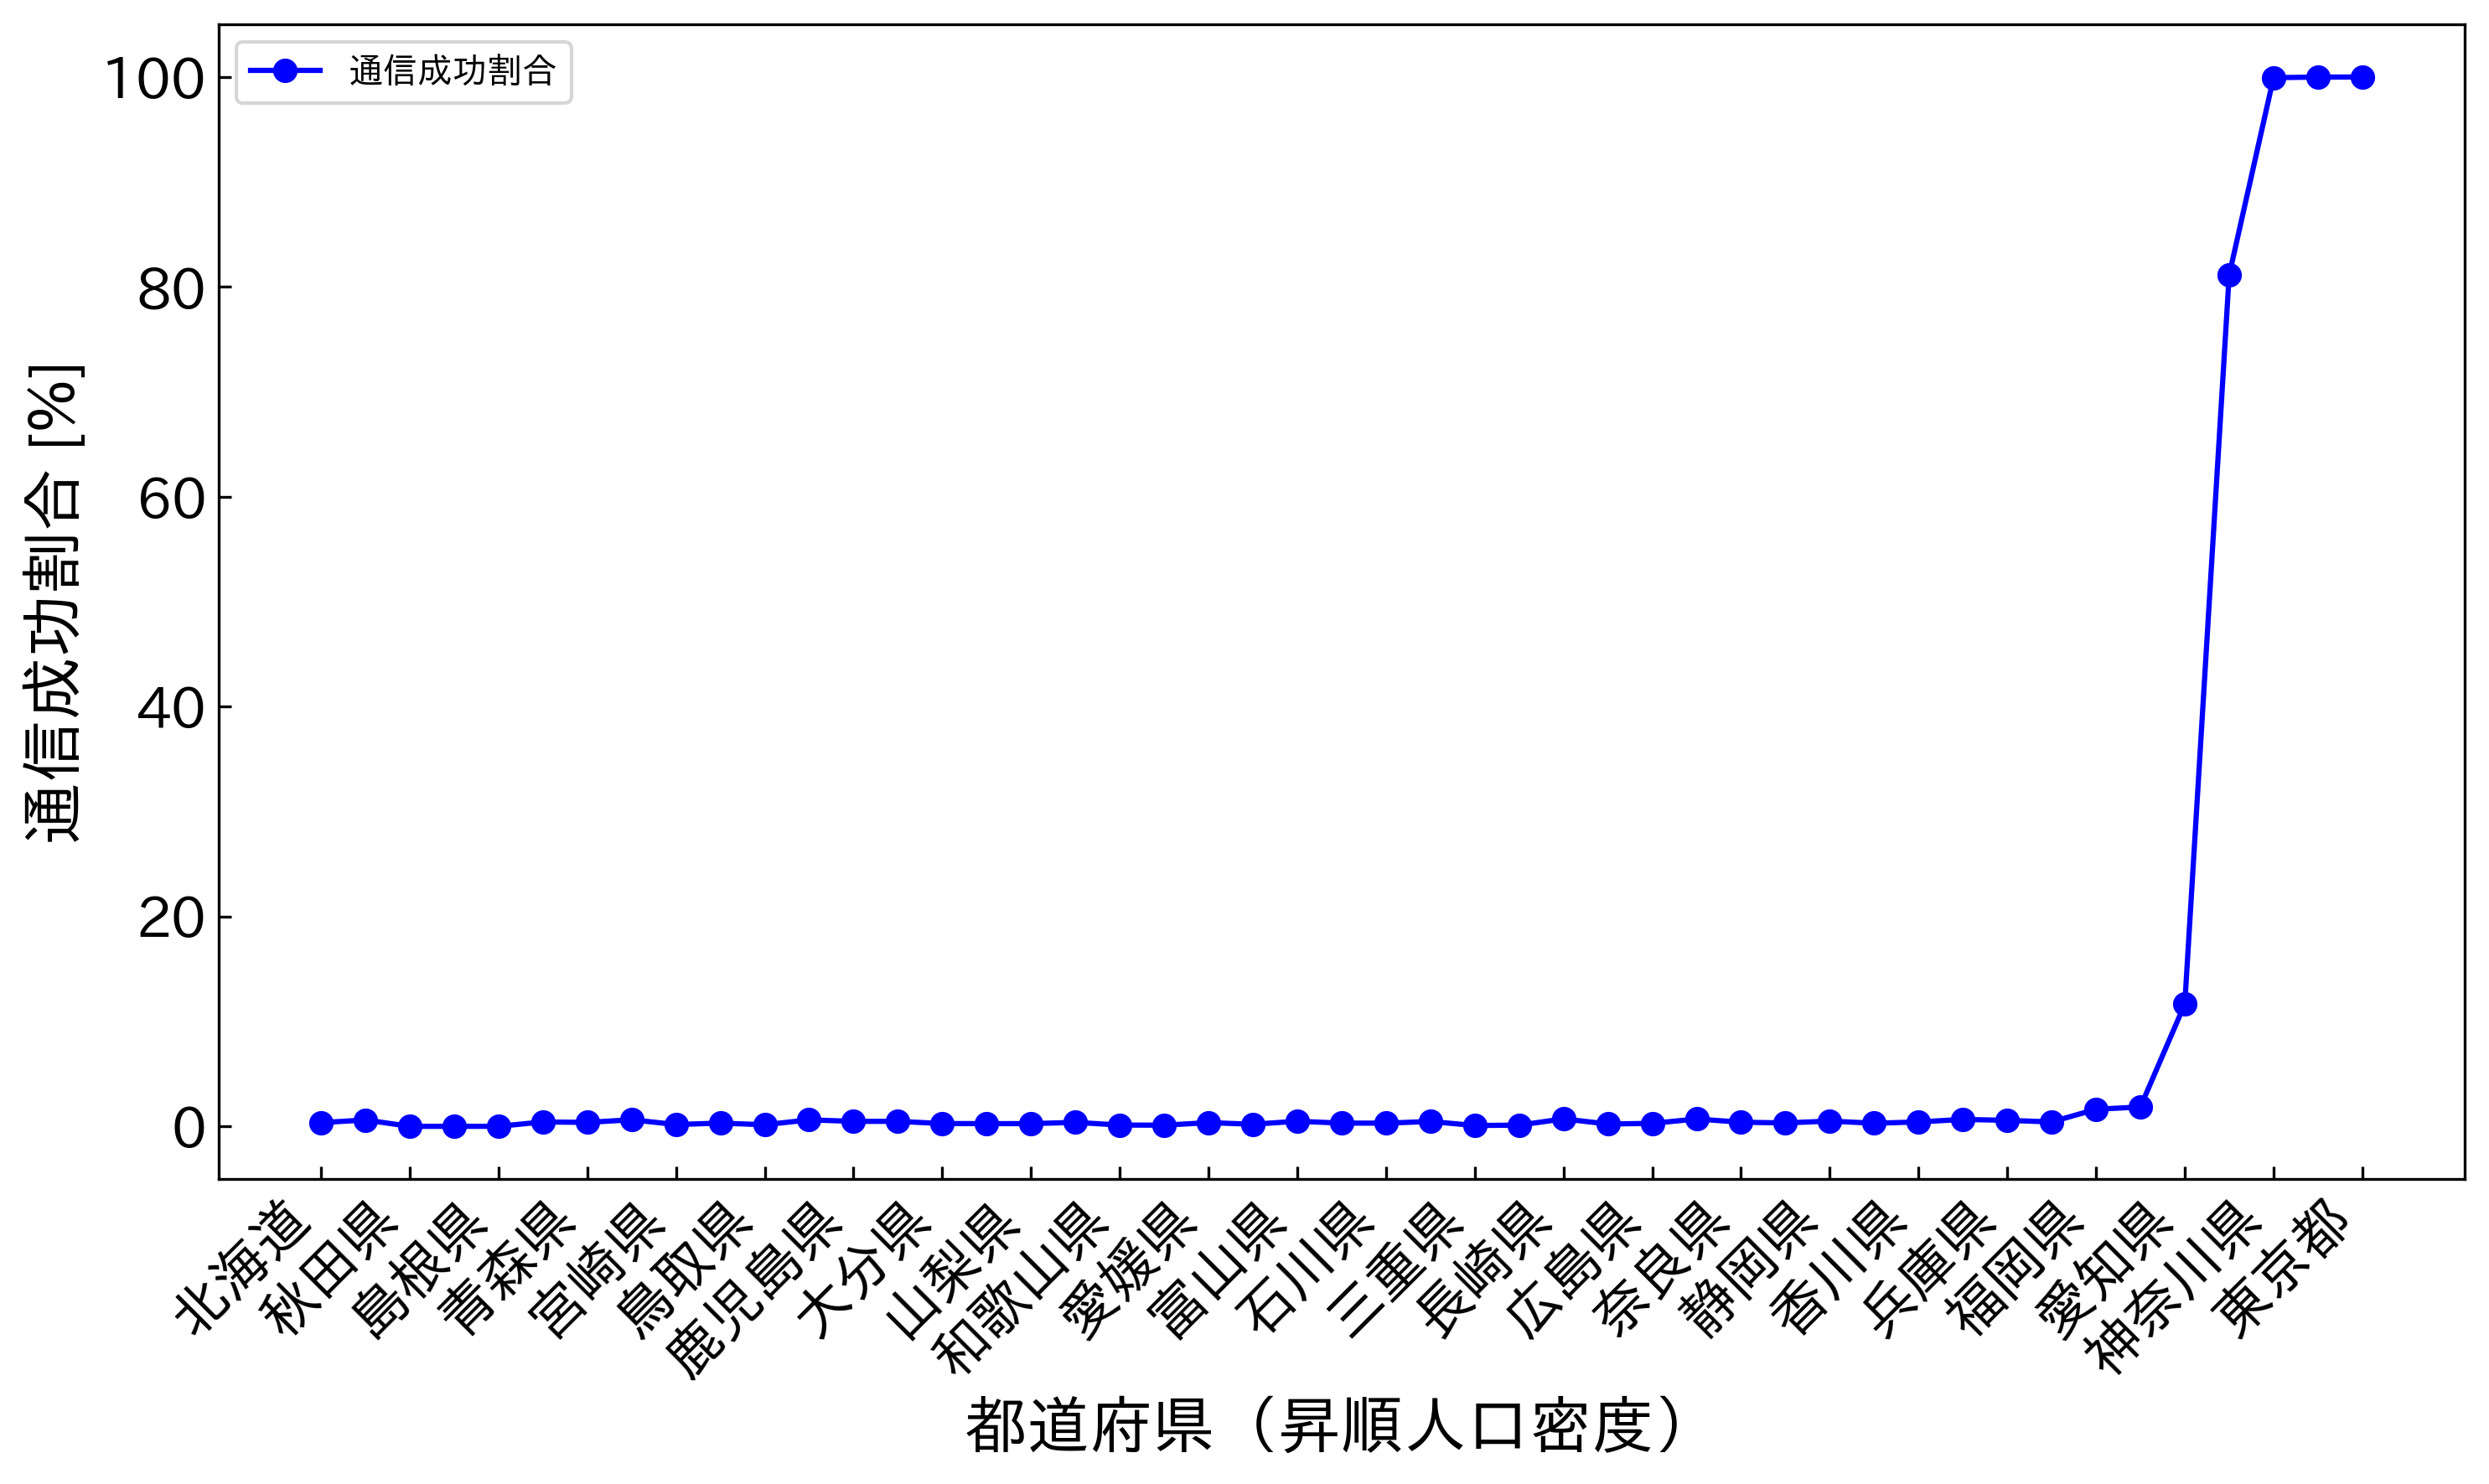
\includegraphics[width=125mm]{通信成功率グラフ.png}
  \caption{各都道府県の通信成功割合}
  \label{figure:各都道府県の通信成功割合}
\end{figure}

\subsection{人口密度が高い地域の場合}
・人口密度が高い地域に対して閾値$X$の値を変化させ,通信成功割合が最も高い$X$を確認する.
・おそらく,人口密度が大きくなると$X$の値が増加する方向にシフトすると思われる.

\subsection{人口密度が低い地域の場合}

%---考察---------------------------------------------------------------------------------------
\clearpage
\section{考察}

%---まとめ---------------------------------------------------------------------------------------
\section{まとめ}

%---今後の課題---------------------------------------------------------------------------------------
\section{今後の課題}

%---参考文献()---------------------------------------------------------------------------------------
\clearpage
\addcontentsline{toc}{section}{参考文献}
\bibliographystyle{junsrt}
\bibliography{arxiv}


\end{document}